% ========================================
%	Header einbinden
% ========================================

\documentclass[bibtotoc,titlepage]{scrartcl}

% Deutsche Spracheinstellungen
\usepackage[ngerman,german]{babel, varioref}
\usepackage[T1]{fontenc}
\usepackage[utf8]{inputenc}

%\usepackage{marvosym}

\usepackage{amsfonts}
\usepackage{amssymb}
\usepackage{amsmath}
\usepackage{amscd}
\usepackage{amstext}

\usepackage{longtable}

%\usepackage{bibgerm}

\usepackage{footnpag}

\usepackage{ifthen}                 %%% package for conditionals in TeX
\usepackage[amssymb]{SIunits}
%Für textumflossene Bilder und Tablellen
%\usepackage{floatflt} - veraltet

%Für Testzwecke aktivieren, zeigt labels und refs im Text an.
%\usepackage{showkeys}

% Abstand zwischen zwei Absätzen nach DIN (1,5 Zeilen)
% \setlength{\parskip}{1.5ex plus0.5ex minus0.5ex}

% Einrückung am Anfang eines neuen Absatzes nach DIN (keine)
%\setlength{\parindent}{0pt}

% Ränder definieren
% \setlength{\oddsidemargin}{0.3cm}
% \setlength{\textwidth}{15.6cm}

% bessere Bildunterschriften
%\usepackage[center]{caption2}


% Problemlösungen beim Umgang mit Gleitumgebungen
\usepackage{float}

% Nummeriert bis zur Strukturstufe 3 (also <section>, <subsection> und <subsubsection>)
%\setcounter{secnumdepth}{3}

% Führt das Inhaltsverzeichnis bis zur Strukturstufe 3
%\setcounter{tocdepth}{3}
\usepackage[version=3]{mhchem}
	\mhchemoptions{minus-sidebearing-left=0.06em, minus-sidebearing-right=0.11em}
\usepackage{exscale}

\newenvironment{dsm} {\begin{displaymath}} {\end{displaymath}}
\newenvironment{vars} {\begin{center}\scriptsize} {\normalsize \end{center}}


\newcommand {\en} {\varepsilon_0}               % Epsilon-Null aus der Elektrodynamik
\newcommand {\lap} {\; \mathbf{\Delta}}         % Laplace-Operator
\newcommand {\R} { \mathbb{R} }                 % Menge der reellen Zahlen
\newcommand {\e} { \ \mathbf{e} }               % Eulersche Zahl
\renewcommand {\i} { \mathbf{i} }               % komplexe Zahl i
\newcommand {\N} { \mathbb{N} }                 % Menge der nat. Zahlen
\newcommand {\C} { \mathbb{C} }                 % Menge der kompl. Zahlen
\newcommand {\Z} { \mathbb{Z} }                 % Menge der kompl. Zahlen
\newcommand {\limi}[1]{\lim_{#1 \rightarrow \infty}} % Limes unendlich
\newcommand {\sumi}[1]{\sum_{#1=0}^\infty}
\newcommand {\rot} {\; \mathrm{rot} \,}         % Rotation
\newcommand {\grad} {\; \mathrm{grad} \,}       % Gradient
\newcommand {\dive} {\; \mathrm{div} \,}        % Divergenz
\newcommand {\dx} {\; \mathrm{d} }              % Differential d
\newcommand {\cotanh} {\; \mathrm{cotanh} \,}   %Cotangenshyperbolicus
\newcommand {\asinh} {\; \mathrm{areasinh} \,}  %Area-Sinus-Hyp.
\newcommand {\acosh} {\; \mathrm{areacosh} \,}  %Area-Cosinus-H.
\newcommand {\atanh} {\; \mathrm{areatanh} \,}  %Area Tangens-H.
\newcommand {\acoth} {\; \mathrm{areacoth} \,}  % Area-cotangens
\newcommand {\Sp} {\; \mathrm{Sp} \,}
\newcommand {\mbe} {\stackrel{\text{!}}{=}}     %Must Be Equal
\newcommand{\qed} { \hfill $\square$\\}
\renewcommand{\i} {\imath}
\def\captionsngerman{\def\figurename{\textbf{Abb.}}}

%%%%%%%%%%%%%%%%%%%%%%%%%%%%%%%%%%%%%%%%%%%%%%%%%%%%%%%%%%%%%%%%%%%%%%%%%%%%
% SWITCH FOR PDFLATEX or LATEX
%%%%%%%%%%%%%%%%%%%%%%%%%%%%%%%%%%%%%%%%%%%%%%%%%%%%%%%%%%%%%%%%%%%%%%%%%%%%
%%%
\ifx\pdfoutput\undefined %%%%%%%%%%%%%%%%%%%%%%%%%%%%%%%%%%%%%%%%% LATEX %%%
%%%
\usepackage[dvips]{graphicx}       %%% graphics for dvips
\DeclareGraphicsExtensions{.eps,.ps}   %%% standard extension for included graphics
\usepackage[ps2pdf]{thumbpdf}      %%% thumbnails for ps2pdf
\usepackage[ps2pdf,                %%% hyper-references for ps2pdf
bookmarks=true,%                   %%% generate bookmarks ...
bookmarksnumbered=true,%           %%% ... with numbers
hypertexnames=false,%              %%% needed for correct links to figures !!!
breaklinks=true,%                  %%% breaks lines, but links are very small
linkbordercolor={0 0 1},%          %%% blue frames around links
pdfborder={0 0 112.0}]{hyperref}%  %%% border-width of frames
%                                      will be multiplied with 0.009 by ps2pdf
%
\hypersetup{ pdfauthor   = {Hannes Franke; Julius Tilly},
pdftitle    = {V301 Innenwiderstand und Leistungsanpassung}, pdfsubject  = {Protokoll FP}, pdfkeywords = {V301, Innenwiderstand, Leistungsanpassung},
pdfcreator  = {LaTeX with hyperref package}, pdfproducer = {dvips
+ ps2pdf} }
%%%
\else %%%%%%%%%%%%%%%%%%%%%%%%%%%%%%%%%%%%%%%%%%%%%%%%%%%%%%%%%% PDFLATEX %%%
%%%
\usepackage[pdftex]{graphicx}      %%% graphics for pdfLaTeX
\DeclareGraphicsExtensions{.pdf}   %%% standard extension for included graphics
\usepackage[pdftex]{thumbpdf}      %%% thumbnails for pdflatex
\usepackage[pdftex,                %%% hyper-references for pdflatex
bookmarks=true,%                   %%% generate bookmarks ...
bookmarksnumbered=true,%           %%% ... with numbers
hypertexnames=false,%              %%% needed for correct links to figures !!!
breaklinks=true,%                  %%% break links if exceeding a single line
linkbordercolor={0 0 1},
linktocpage]{hyperref} %%% blue frames around links
%                                  %%% pdfborder={0 0 1} is the default
\hypersetup{
pdftitle    = {V301 Innenwiderstand und Leistungsanpassung}, 
pdfsubject  = {Protokoll AP}, 
pdfkeywords = {V301, Innenwiderstand, Leistungsanpassung},
pdfsubject  = {Protokoll AP},
pdfkeywords = {V301, Innenwiderstand, Leistungsanpassung}}
%                                  %%% pdfcreator, pdfproducer,
%                                      and CreationDate are automatically set
%                                      by pdflatex !!!
\pdfadjustspacing=1                %%% force LaTeX-like character spacing
\usepackage{epstopdf}
%
\fi %%%%%%%%%%%%%%%%%%%%%%%%%%%%%%%%%%%%%%%%%%%%%%%%%%% END OF CONDITION %%%
%%%%%%%%%%%%%%%%%%%%%%%%%%%%%%%%%%%%%%%%%%%%%%%%%%%%%%%%%%%%%%%%%%%%%%%%%%%%
% seitliche Tabellen und Abbildungen
%\usepackage{rotating}
\usepackage{ae}
\usepackage{
  array,
  booktabs,
  dcolumn
}
\makeatletter 
  \renewenvironment{figure}[1][] {% 
    \ifthenelse{\equal{#1}{}}{% 
      \@float{figure} 
    }{% 
      \@float{figure}[#1]% 
    }% 
    \centering 
  }{% 
    \end@float 
  } 
  \makeatother 


  \makeatletter 
  \renewenvironment{table}[1][] {% 
    \ifthenelse{\equal{#1}{}}{% 
      \@float{table} 
    }{% 
      \@float{table}[#1]% 
    }% 
    \centering 
  }{% 
    \end@float 
  } 
  \makeatother 
%\usepackage{listings}
%\lstloadlanguages{[Visual]Basic}
%\allowdisplaybreaks[1]
%\usepackage{hycap}
%\usepackage{fancyunits}


% ========================================
%	Angaben für das Titelblatt
% ========================================

\title{Versuch 101 - Das Trägheitsmoment\\				% Titel des Versuchs 
\large TU Dortmund, Fakultät Physik\\ 
\normalsize Anfänger-Praktikum}

\author{Jan Adam\\			% Name Praktikumspartner A
{\small \href{jan.adam@tu-dortmund.de}{jan.adam@tu-dortmund.de}}	% Erzeugt interaktiven einen Link
\and						% um einen weiteren Author hinzuzfügen
Dimitrios Skodras\\					% Name Praktikumspartner B
{\small \href{dimitrios.skodras@tu-dortmund.de}{dimitrios.skodras@tu-dortmund.de}}		% Erzeugt interaktiven einen Link
}
\date{30.April 2013}				% Das Datum der Versuchsdurchführung

% ========================================
%	Das Dokument beginnt
% ========================================

\begin{document}

% ========================================
%	Titelblatt erzeugen
% ========================================

\maketitle					% Jetzt wird die Titelseite erzeugt
\thispagestyle{empty} 				% Weder Kopfzeile noch Fußzeile

% ========================================
%	Der Vorspann
% ========================================

%\newpage					% Wenn Verzeichnisse auf einer neuen Seite beginnen sollen
%\pagestyle{empty}				% Weder Kopf- noch Fußzeile für Verzeichnisse

\tableofcontents

%\newpage					% eine neue Seite
%\thispagestyle{empty}				% Weder Kopf- noch Fußzeile für Verzeichnisse
%\listoffigures					% Abbildungsverzeichnis

%\newpage					% eine neue Seite
%\thispagestyle{empty}				% Weder Kopf- noch Fußzeile für Verzeichnisse
%\listoftables					% Tabellenverzeichnis
\newpage					% eine neue Seite


% ========================================
%	Kapitel
% ========================================

\section{Einleitung}
Im Zuge dieses Experiments wird das Trägheitsmoment von Körpern, sowie einer Holzpuppe in zwei verschiedenen Positionen bestimmt. 
Weiterhin soll der Satz von Steiner geprüft werden.

\section{Theorie}
Charakteristisch für die Dynamik von Rotationsbewegungen sind die Größen Drehmoment $M$, Trägheitsmoment $I$ und Winkelbeschleunigung
$\dot \omega$. Das Trägheitsmoment einer punktförmigen masse ist durch $I = m\,r^2$ gegeben. Entsprechend bei ausgedehnten Körpern, bei
denen sich die Massenelemente um eine feste Achse drehen, werden die einzelnen Trägheitsmomente aufsummiert
\begin{align}
 I = \sum_i r^2_i\,m_i.
\end{align}
Bei einer kontinuierlichen Massenverteilung gilt allgemein
\begin{align}
 I = \int r^2 \dx m.
\end{align}
$r$ beschreibt hierbei den Abstand des Massepunkts zur Drehachse. Daher ist das Trägheitsmoment einfacher, symmetrischer Körper leicht
bestimmbar, das komplexerer Körper durch Summation einzelner Trägheitsmomente. Sofern die Drehachse aber nicht mit einem betrachteten
Körper übereinstimmt, sondern um eine Strecke $a$ parallel zu ihr verschoben ist, so kann der Satz von Steiner Abhilfe schaffen
\begin{align}
 I = I_s + m \cdot a^2,
\end{align}
wobei $I_s$ das Trägheitsmoment bezüglich der Drehachse durch den Schwerpunkt ist. 

Bei Rotationsbewegungen von Körpern ist das Drehmoment durch $M = \vec{F} \times \vec{r}$ gegeben. Wenn nun ein schwingbarer Körper
durch eine Auslenkung um den Winkel $\varphi$ aus seiner Ruhelage gebracht wird, wirkt eine Feder ein rücktreibendes Drehmoment auf ihn.
Die Schwingungdauer des Körpers $T$ ist durch sein Trägheitsmoment $I$ und die zu bestimmende Winkelrichtgröße $D$ gegeben
\begin{align}
 T = 2\pi \sqrt{\frac{I}{D}}.
 \label{eq_periode}
\end{align}
Das Drehmoment ist mit der Winkelrichtgröße über den Auslenkwinkel verknüpft
\begin{align}
 D = \frac{M}{\varphi}.
 \label{eq_winkel}
\end{align}

\section{Durchführung}
In Abbildung \eqref{pic_aufbau} ist der Aufbau skizziert. Der zu untersuchende Körper ist mit einer Feder gekoppelt, deren Winkelrichtgröße
es zu bestimmen gilt. Wenn man eine Federwaage senkrecht zum Radius der vom Körper beschriebenen Kreisbahn mit einem Haken an der Stange
in einem bestimmten Abstand $r$ ansetzt, misst man für eine Auslenkung $\varphi$ eine Kraft $F$. Mit der vorausgesetzten Orthogonalität
des Kraft- und Ortsvektors, kann man die Winkelrichtgröße nach \eqref{eq_winkel} berechnen
\begin{align}
 D = \frac{F\cdot r}{\varphi}.
\end{align}

\begin{figure}[H]
 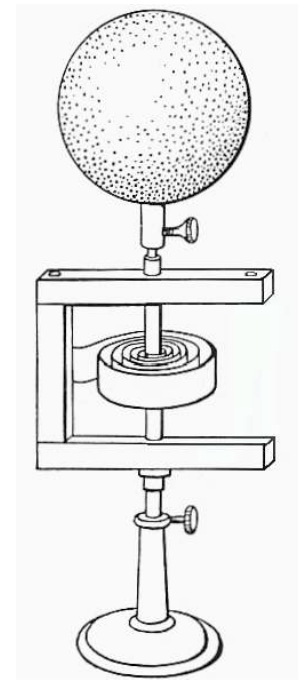
\includegraphics[width=0.3\textwidth]{pics/aufbau.png}
 \caption{Experimenteller Versuchsaufbau (aus Versuchsanleitung)}
 \label{pic_aufbau}
\end{figure}

Selbst ohne Körper hat die Drillachse ein Eigenträgheitsmoment $I_D$, welches über eine massearme Stange mit zwei Gewichten in Abstand $a$
, welche senkrecht zur Achse angebracht, ermittelt werden kann. Das System, in Schwingung gebracht, oszilliert harmonisch mit einer 
zu messenden Periodendauer $T$. Nach \eqref{eq_periode} kann $I_D$ bestimmt werden.

Das Trägheitsmoment zweier verschiedener Zylinder wird ebenfalls durch Messung von Periodendauer, sowie Ausdehnungen und Masse bestimmt.
\eqref{eq_periode} liefert ebenfalls die Lösung.

Für eine Holzpuppe soll das Trägheitsmoment in zwei Stellungen (vergleiche Abbildung \ref{pic_puppe}) berechnet werden. Hierbei werden
die einzelnen Bestandteile als Zylinder angenähert und ihre einzelnen Trägheitsmomente aufsummiert.

\begin{figure}[H]
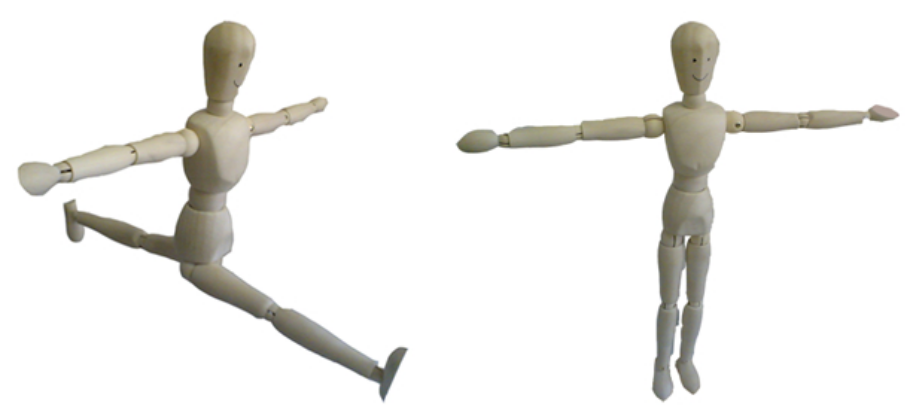
\includegraphics[width=0.8\textwidth]{pics/puppe.png}
\caption{Verwandte Stellungen der Holzpuppe (101 - Trägheitsmomente starrer Körper)}
\label{pic_puppe}
\end{figure}






\section{Auswertung}
\subsection{Winkelrichtgröße und Eigenträgheitsmoment}
Zur Bestimmung der Winkelrichtgröße wird die Feder mit der Querstange daran um verschiedene Winkel ausgelenkt und mittels einer Federwaage die Rückstellkraft bestimmt.\\
Gemessen wurden folgende Werte:
\begin{table}[htbp]
\begin{tabular}{|c|c|}
\hline 
Winkel [Grad]&	Kraft [Newton]\\ \hline
20	&0,13\\ \hline
40	&0,16\\ \hline
60	&0,21\\ \hline
80	&0,23\\ \hline
100	&0,29\\ \hline
120	&0,34\\ \hline
140	&0,39\\ \hline
160	&0,43\\ \hline
180	&0,48\\ \hline
200	&0,55\\ \hline
220	&0,60\\ \hline
\end{tabular} 
\caption{Messung der Rückstellkraft im Abstand 20cm zur Drehachse}
\end{table}

Mit Gleichung \eqref{eq_winkel} ergibt sich daraus eine Winkelrichtgröße des Aufbaus von:
\begin{align*}
D=0.072 \pm0.023
\end{align*}


Um Eigenträgheit der Drillachse $I_D$ zu bestimmen, ersetzt man das Trägheitsmoment I in Gleichung \eqref{eq_periode} durch
\begin{align*}
I&=I_D+I_{Stab}+I_{Zylinder} \qquad \text{, wobei}\\
I_{Zylinder}&=2m\cdot\left(\frac{R^2}{4}+\frac{l^2}{12}\right)
\end{align*}
das Trägheitsmoment der beiden Zylinder inklusive dem Betrag durch den Satz von Steiner beschreibt.
Quadriert man die Gleichung und stellt diese um, so erhält man:
\begin{align}
T^2=\frac{8m\pi^2}{D}\cdot a^2 + \frac{4\pi}{D}  \left[  I_D+I_{Stab}+2m\left(\frac{R^2}{4}+\frac{l^2}{12}\right)\right]
\end{align}

\begin{table}[htbp]
\begin{tabular}{|c|c|}
\hline
Abstand [m] &	t [s]\\ \hline
0.02&	10.565\\ \hline
0.04&	11.85\\ \hline
0.06&	13.185\\ \hline
0.08&	15.56\\ \hline
0.10&	17.01\\ \hline
0.12&	19.225\\ \hline
0.14&	21.43\\ \hline
0.16&	23.47\\ \hline
0.18&	25.665\\ \hline
0.20&	28.05\\ \hline
\end{tabular} 
\caption{Messwerte bei schwingenden Massen, die Zeiten sind bereits gemittelt}
\end{table}

Plottet man nun $T^2$ gegen $a^2$, so erhält man eine Gerade, mit:
\begin{figure}[htbp]
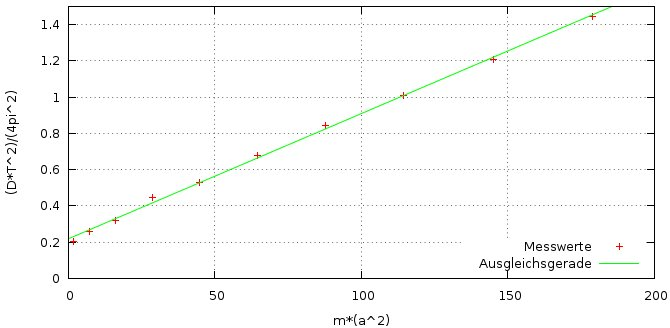
\includegraphics[width=0.8\textwidth]{pics/eigentr.jpg}
\end{figure}
\begin{align*}
\text{Steigung:} \qquad m&=\frac{8m\pi^2}{D}=16843.9 \pm 234.6\\
\text{Y-Achsenabschnitt }\qquad b&=\frac{4\pi}{D}  \left[  I_D+I_{Stab}+2m\left(\frac{R^2}{4}+\frac{l^2}{12}\right)\right]s=118.86 \pm 4.72
\end{align*}

Dadurch erhält man einen weiteren Wert für die Winkelrichtgröße
\begin{align*}
D'=(1,0481\pm 0,0115) \cdot10^{-3}
\end{align*}
Und es kann erstmals das Eigenträgheitsmoment der Drillachse bestimmt werden (mit dem ungestrichenen D)
\begin{align*}
I_D=0,22 \pm 0,07
\end{align*}

\subsection{Trägheitsmoment zweier Zylinder}
Als nächstes soll das Trägheitsmoment zweier Zylinder berechnet und anschließend mit den gemessenen Werten verglichen werden.

Das Trägheitsmoment eines Zylinders durch seine Symmetrieachse berechnet sich zu:

\begin{align}
I_{Z}=\frac{mR^2}{2}
\label{eq_Izyl}
\end{align}

Die Zylinder haben folgende Daten:
\begin{table}[htbp]
\begin{tabular}{|c|c|c|c|}
\hline 
 & Höhe [m] & Radius [m] & Gewicht [kg]\\ 
\hline 
Zylinder 1 & 0,1008 & 0,04965 & 0,36864 \\ 
\hline 
Zylinder 2 & 0,0302 & 0,0371 & 1,2728 \\ 
\hline 
\end{tabular} 
\caption{}
\end{table}

Eingesetzt in Gleichung \eqref{eq_Izyl} ergibt dies:
\begin{align*}
I_{Zyl 1}&=(4,5437\pm0,0092)\cdot10^{-4}\\
I_{Zyl 2}&=(8,76\pm0,036)\cdot10^{-4}
\end{align*}

Berechnet man das Trägheitsmoment über Gleichung \eqref{eq_periode}, so benötigt man die Schwingzeit der Zylinder:
\begin{table}[htbp]
\begin{tabular}{|c|c|}
\hline 
$t_1$ [s] & $t_2$ [s]\\ \hline
0.74&	1.34\\ \hline
0.73&	1.33\\ \hline
0.76&	1.33\\ \hline
0.74&	1.32\\ \hline
0.75&	1.32\\ \hline
0.73&	1.35\\ \hline
0.73&	1.33\\ \hline
0.75&	1.30\\ \hline
0.73&	1.33\\ \hline
0.74&	1.31\\ \hline
\end{tabular} 
\caption{Die Zeiten wurden über fünf Perioden gemittelt}
\end{table}
\newpage
Die Werte ergeben:
\begin{align*}
t_{Zyl 1}&=0.739 \pm 0.010\\
I'_{Zyl 1}&=(1,0027\pm0,69)\cdot10^{-3}\\
\end{align*}
\begin{align*}
t_{Zyl 2}&=1.325 \pm  0.014\\
I'_{Zyl 1}&=(3,2219312\pm5,86)\cdot10^{-3}
\end{align*}

\subsection{Trägheitsmoment einer Puppe}
Zum Schluss soll das Trägheitsmoment einer Puppe bestimmt werden. Die Gliedmaßen werden dabei als Zylinder angenährt und ihr Umfang wird an 10 verschiedenen Stellen gemessen, um einen präzisen Mittelwert zu erhalten.
\begin{table}[htbp]
\begin{tabular}{|c|c|c|c|c|}
\hline 		
&	Bein&	Arm	&Oberkörper	&Kopf	\\ \hline	
Durchmesser [m]&	0.01643&	0.01403&	0.03337&	0.02113\\ \hline				
Länge [m] &	0.1539	&0.138	&0.1	&0.0548\\ \hline	
					
Volumen [$m^3$]	&0.000032629	&0.0000213346	&0.000087459	&0.000019216	\\ \hline	
Anteil am Gesamtvolumen	&0.203	&0.133	&0.5444	&0.120	\\ \hline		
Masse [kg]	&0.0326618101	&0.0213560501	&0.0875465257	&0.0192356141\\ \hline
Abstand [m]	&0.0218	&0.1678	&&\\ \hline	
					
Trägheit&	0.000001102	&0.000034155&	0.000012186	&0.0000010735\\ \hline	
TrägheitSteiner	&0.0000155222	&0.0006013189	&&	\\ \hline	
\end{tabular} 
\caption{Puppe mit ausgestreckten Armen}
\end{table}

Summiert man alle Teilträgheiten und die beiden Terme, die durch den Satz von Steiner entstehen auf, so erhält man als Trägheitsmoment der Puppe:
\begin{align*}
I_{Puppe 1}= 0.001317
\end{align*}

\begin{table}[htbp]
\begin{tabular}{|c|c|c|c|c|}
\hline 		
&	Bein&	Arm	&Oberkörper	&Kopf	\\ \hline	
Durchmesser [m]	&0.01643&	0.01403	&0.03337	&0.02113	\\ \hline		
Länge [m]	&0.1539	&0.138	&0.1	&0.0548\\ \hline	
Volumen [$m^3$]	&0.000032629	&0.0000213346	&0.0000874586	&0.0000192163\\ \hline	
VolGes [$m^3$]	&0.0001606384	&&&		\\ \hline	
Anteil am Gesamtvolumen&	0.203	&0.133&	0.544	&0.120\\ \hline
Masse [kg]	&0.0326618101&	0.0213560501	&0.0875465257	&0.0192356141\\ \hline	
Abstand [m]&	0.093635	&0.1678&&\\ \hline	
Trägheit&	0.000066671&	0.0000341548&	0.000012186&	0.000001074\\ \hline	
TrägheitSteiner&	0.0002863629&	0.0006013189&&	\\ \hline	
\end{tabular} 
\caption{Puppe mit ausgestreckten Armen und Beinen}
\end{table}

Man erhält als Trägheitsmoment der Puppe:
\begin{align*}
I_{Puppe 2}=0.00199
\end{align*}

Zum Vergleich kann man die Trägheit immer noch nach Gleichung \eqref{eq_periode} berechnen. Dazu wird die Puppe als langer Zylinder angenährt, indem alle Teilradien mit der Länge des jeweiligen Körperteils gewichtet aufsummiert und dann durch die Höhe der Puppe dividiert wird. Es ergibt sich der Radius:
\begin{align*}
R_{Puppe 1}=1,65cm\\
R_{Puppe 2}=1,70cm
\end{align*}
Und damit das Trägheitsmoment:
\begin{align*}
I'_{Puppe 2}=2,19\cdot10^{-5}\\
I'_{Puppe 2}=2,32\cdot10^{-5}
\end{align*}

\section{Diskussion}
Das Eigenträgheitsmoment der Drehachse lässt sich relativ genau berechnen, dagegen weichen die Werte für die Winkelrichtgröße bei den verschiedenen Auswertmethoden stark von einander ab. Dies ist vermutlich darauf zurückzuführen, dass die Apparatur eine relativ hohe Reibung hat, die sich besonders bei kleinen Auslenkungen bemerkbar macht. Die Gleichung gilt jedoch nur für kleine Winkel, daher ist die Auswertung über die Federwaage aussagekräftiger.

Die Trägheitsmomente der beiden Zylinder liegen um einen Faktor von ungefähr 3 auseinander, wenn man die theoretischen mit den gemessenen Werten vergleicht. Auch dies lässt sich vermutlich darauf zurückführen, dass die Apparatur zu stark gedämpft ist. Die Körper schwingen recht schnell und um den statistischen Fehler zu minimieren muss man über mehrere Schwingungen mitteln. Da die Amplitude jedoch um gut 15\% pro Periode abnimmt, schlägt dieser Fehler dann mehr ins Gewicht.

Bei den Trägheitsmomenten der Puppe merkt man den Unterschied zu den Theoriewerten am deutlichsten. Die Werte liegen eine ganze Größenordnung auseinander. Das die Differenz hier besonders groß ist, hat verschiedene Gründe. Zum einen wirkt wieder die Dämpfung der Apparatur auf die Messung ein. Zum anderen ist die Figur aber auch nicht genau mittig auf ihrer Symmetrie befestigt und ihre Haltung ist relativ instabil. Außerdem ist die Puppe nicht richtig fest auf dem Stab befestigt und rutscht bei größeren Beschleunigungen hin und her.
Bei den Theoriewerten schlägt am härtesten zu Buche, dass die Puppe nur grob aus Zylindern angenährt wurde. Die genaue Mittelung minimiert diesen Fehler zwar, dennoch ist er deutlich zu spüren. Zudem wurden Füße und Hände der Puppe, sowie der Metallstab völlig vernachlässigt.

Das die Messwerte dennoch so nah beieinander liegen, ist als Erfolg zu werten.
% ========================================
%	Literaturverzeichnis
% ========================================

%\bibliographystyle{plainnat}			% Bibliographie-Style auswählen
%\bibliography{BIBDATEI}			% Literaturverzeichnis

% ========================================
%	Das Dokument endent
% ========================================

\end{document}
